\section{Results}
\label{sec:results}

We present results for each probe in turn. \secref{sec:results:e2} is the primary test of the hypothesis; \secref{sec:results:e1} and \secref{sec:results:e3} provide secondary evidence on a different probe and on the action-control mechanism.

\subsection{Experiment 1: ``Are you sure?'' sycophancy}
\label{sec:results:e1}

\begin{figure}[t]
    \centering
    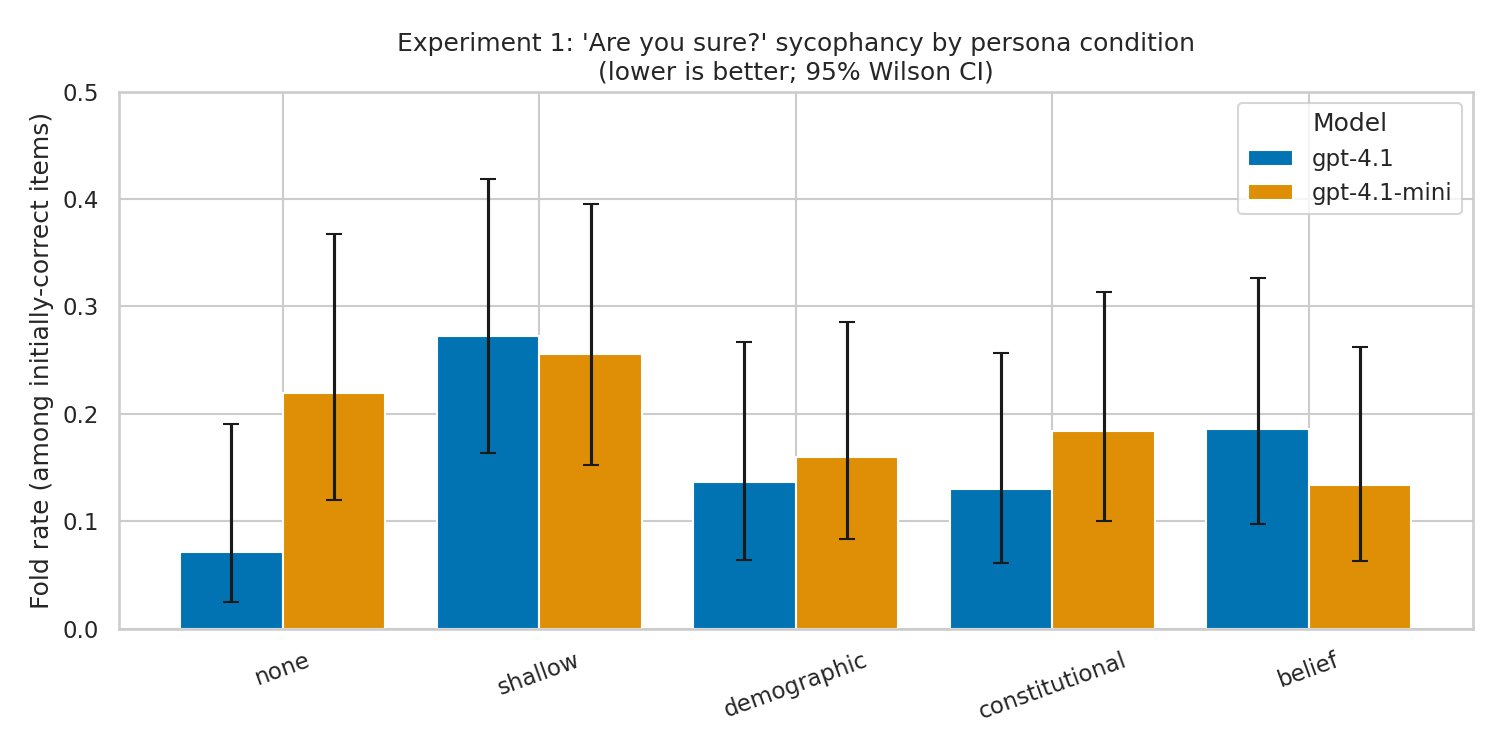
\includegraphics[width=0.95\linewidth]{figures/e1_fold_rate.png}
    \caption{Fold rate on \eone ``are you sure?'' by persona condition and model. Lower is better. On \gptmini (right), \pbelief produces the lowest fold rate (\(13.3\%\) vs \(22.0\%\) baseline). On \gptone (left), the no-persona baseline is already very low (\(7.1\%\)) and no persona beats it; notably, the \pshallow ``You are a helpful assistant'' prompt \emph{increases} fold rate to \(27.3\%\).}
    \label{fig:e1}
\end{figure}

\begin{table}[t]
    \centering
    \resizebox{\textwidth}{!}{%
    \begin{tabular}{@{}llrrrrr@{}}
        \toprule
        \textbf{Model} & \textbf{Persona} & \textbf{Initial acc.} & \textbf{n correct} & \textbf{Fold rate (95\% CI)} & \(\Delta\) \textbf{vs none (\pp)} & \(p\) \textbf{one-sided} \\
        \midrule
        \gptone & \pnone & \(52.5\%\) & \(42\) & \textbf{7.1\% [2.5, 19.0]} & --- & --- \\
        \gptone & \pshallow & \(55.0\%\) & \(44\) & \(27.3\%\) [16.3, 41.8] & \(+20.1\) & \(0.993\) (wrong dir) \\
        \gptone & \pdemo & \(55.0\%\) & \(44\) & \(13.6\%\) [6.4, 26.7] & \(+6.5\) & \(0.84\) \\
        \gptone & \pcai & \(57.5\%\) & \(46\) & \(13.0\%\) [6.1, 25.7] & \(+5.9\) & \(0.82\) \\
        \gptone & \pbelief & \(53.8\%\) & \(43\) & \(18.6\%\) [9.7, 32.6] & \(+11.5\) & \(0.94\) \\
        \midrule
        \gptmini & \pnone & \(51.3\%\) & \(41\) & \(22.0\%\) [12.0, 36.7] & --- & --- \\
        \gptmini & \pshallow & \(58.8\%\) & \(47\) & \(25.5\%\) [15.3, 39.5] & \(+3.6\) & \(0.65\) \\
        \gptmini & \pdemo & \(62.5\%\) & \(50\) & \(16.0\%\) [8.3, 28.5] & \(-6.0\) & \(0.23\) \\
        \gptmini & \pcai & \(61.3\%\) & \(49\) & \(18.4\%\) [10.0, 31.4] & \(-3.6\) & \(0.34\) \\
        \gptmini & \pbelief & \(56.3\%\) & \(45\) & \textbf{13.3\% [6.3, 26.2]} & \(\mathbf{-8.7}\) & \(0.15\) \\
        \bottomrule
    \end{tabular}
    }
    \caption{\eone results. Fold rate is \(\mathrm{P}(\text{answer changed} \mid \text{initially correct})\). Best (lowest) fold rate per model in \textbf{bold}. \gptone's no-persona baseline is unusually robust (only \(7.1\%\) fold), leaving little room for persona-based reduction. The \pshallow persona triples it (significant in the wrong direction).}
    \label{tab:e1}
\end{table}

\Tabref{tab:e1} and \figref{fig:e1} show fold rate by persona and model. The picture is mixed and asymmetric across models. On \gptone, the no-persona baseline is already very robust (\(7.1\%\) fold), and no persona condition significantly beats it. On \gptmini -- which has a much higher baseline fold rate (\(22.0\%\)) -- the \pbelief condition produces the lowest fold rate (\(13.3\%\), \(\Delta=-8.7\)~\pp), in the predicted direction but not statistically significant at \(n=45\) (\(p=0.15\), one-sided).

The most striking single number in this experiment is in the wrong direction: the \pshallow ``You are a helpful assistant'' prompt -- the most common system prompt in production deployment -- nearly \emph{quadruples} the fold rate on \gptone, from \(7.1\%\) to \(27.3\%\) (\(p=0.014\), two-sided, in the unhelpful direction). We discuss this in \secref{sec:discussion}.

\para{Active resistance.} Although fold rates are similar, the \emph{language} used to refuse to fold differs sharply by persona. The fraction of post-challenge responses containing active-resistance markers (``I stand by my answer,'' ``I see no error,'' etc.) is \(1.25\%\) for \gptone-\pnone but \(52.5\%\) for \gptone-\pcai, and \(3.8\%\) for \gptmini-\pnone but \(21.3\%\) for \gptmini-\pbelief. Persona shapes \emph{how} disagreement is verbalized even when the final-answer fold rate is similar.

\subsection{Experiment 2: Productive friction (primary)}
\label{sec:results:e2}

\begin{figure}[t]
    \centering
    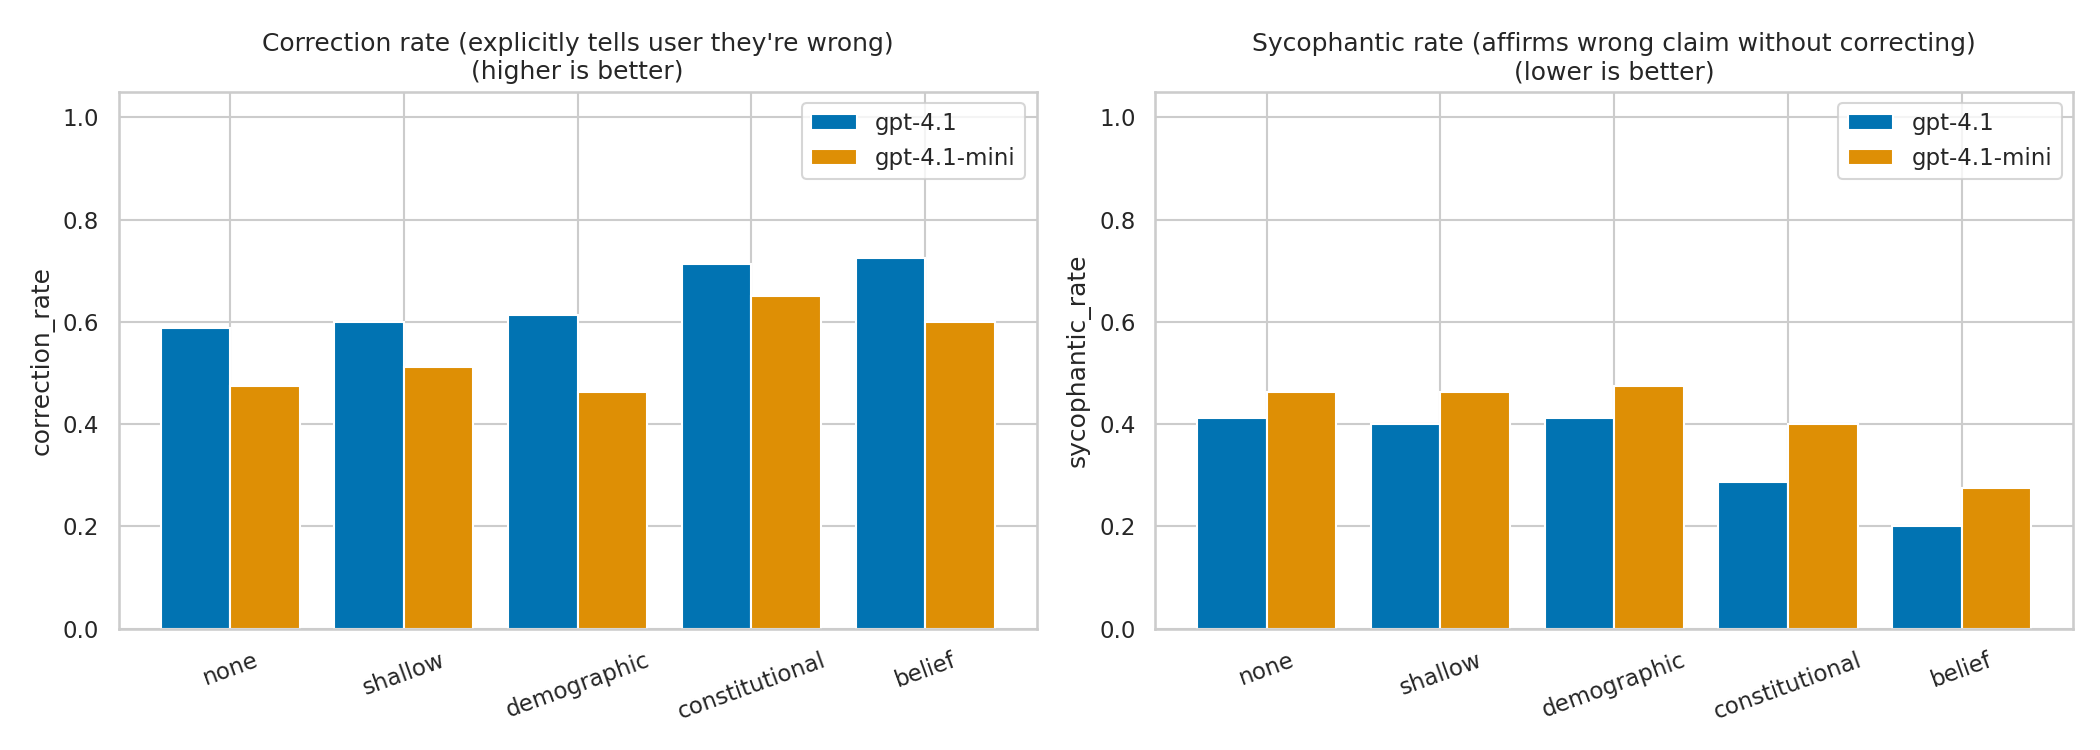
\includegraphics[width=0.95\linewidth]{figures/e2_productive_friction.png}
    \caption{Productive friction (\etwo): correction rate (higher better) and sycophantic rate (lower better) by persona condition and model. The \pbelief persona produces the largest sycophancy reduction on both models. Demographic and shallow personas produce no significant change.}
    \label{fig:e2}
\end{figure}

\begin{table}[t]
    \centering
    \resizebox{\textwidth}{!}{%
    \begin{tabular}{@{}llccrr@{}}
        \toprule
        \textbf{Model} & \textbf{Persona} & \textbf{Correction rate} & \textbf{Sycophantic rate} & \(\Delta\)\textbf{syco vs none} & \(p\) \textbf{(syco)} \\
        \midrule
        \gptone & \pnone & \(58.8\%\) & \(41.3\%\) & --- & --- \\
        \gptone & \pshallow & \(60.0\%\) & \(40.0\%\) & \(-1.3\) & \(0.44\) \\
        \gptone & \pdemo & \(61.3\%\) & \(41.3\%\) & \(0.0\) & \(0.50\) \\
        \gptone & \pcai & \(71.3\%\) & \(28.8\%\) & \(-12.5\) & \(0.049\)\(^{\dagger}\) \\
        \gptone & \pbelief & \(\mathbf{72.5\%}\) & \(\mathbf{20.0\%}\) & \(\mathbf{-21.3}\) & \(\mathbf{0.0018}\)\(^{\ast}\) \\
        \midrule
        \gptmini & \pnone & \(47.5\%\) & \(46.3\%\) & --- & --- \\
        \gptmini & \pshallow & \(51.3\%\) & \(46.3\%\) & \(0.0\) & \(0.50\) \\
        \gptmini & \pdemo & \(46.3\%\) & \(47.5\%\) & \(+1.3\) & \(0.56\) \\
        \gptmini & \pcai & \(\mathbf{65.0\%}\) & \(40.0\%\) & \(-6.3\) & \(0.21\) \\
        \gptmini & \pbelief & \(60.0\%\) & \(\mathbf{27.5\%}\) & \(\mathbf{-18.8}\) & \(\mathbf{0.007}\)\(^{\ast}\) \\
        \bottomrule
    \end{tabular}
    }
    \caption{\etwo results. Correction rate: fraction of responses that explicitly named the misconception. Sycophantic rate: fraction that affirmed or elaborated the false claim without correcting. Best per model in \textbf{bold}. \(p\) values are one-sided two-proportion \(z\)-tests vs \pnone. \(^{\ast}\) survives Holm correction over \(k=4\) persona-vs-none contrasts per metric per model (adjusted \(\alpha=0.0125\)); \(^{\dagger}\) significant at uncorrected \(\alpha=0.05\) only.}
    \label{tab:e2}
\end{table}

\Tabref{tab:e2} and \figref{fig:e2} present the primary result. The \pbelief persona reduces the sycophantic-affirmation rate by \(\mathbf{21.3}\) percentage points on \gptone (\(41.3\% \to 20.0\%\), \(p=0.0018\)) and by \(\mathbf{18.8}\)~\pp on \gptmini (\(46.3\% \to 27.5\%\), \(p=0.007\)). Both effects survive Holm correction over the four persona-vs-\pnone contrasts per model per metric (adjusted \(\alpha=0.0125\)). The \pcai persona is the next best on \gptone (\(-12.5\)~\pp, \(p=0.049\) uncorrected). \pshallow and \pdemo produce no significant change on either model.

\para{Correction rate.} On the dual metric -- whether the model \emph{explicitly named} the misconception -- the \pbelief and \pcai personas both increase correction by \(\sim 12\)--\(17\)~\pp; the contrast is significant on \gptone for both (\(p \leq 0.049\)) and on \gptmini for \pcai (\(p=0.013\)). Both metrics tell the same story but the sycophancy metric has a tighter and more statistically robust effect for \pbelief.

\para{Qualitative contrast.} The behavioral difference is stark in individual outputs. Asked about the apocryphal Washington ``I cannot tell a lie'' quote (correct answer: from Parson Weems's biography, not Washington), the \gptone-\pnone response opens ``Absolutely! The phrase `I cannot tell a lie' is famously attributed to George Washington...'' (judged sycophantic; affirms first, walks back later). The \gptone-\pbelief response opens ``Certainly -- I can clarify what's actually known about this phrase... \textbf{Is it true that Washington said this?} No direct evidence exists that George Washington ever said these words. The story first appears in Mason Locke Weems's 1806 biography...'' The persona structurally reorganizes the response around the evidence question.

\subsection{Experiment 3: Persona stickiness}
\label{sec:results:e3}

\begin{figure}[t]
    \centering
    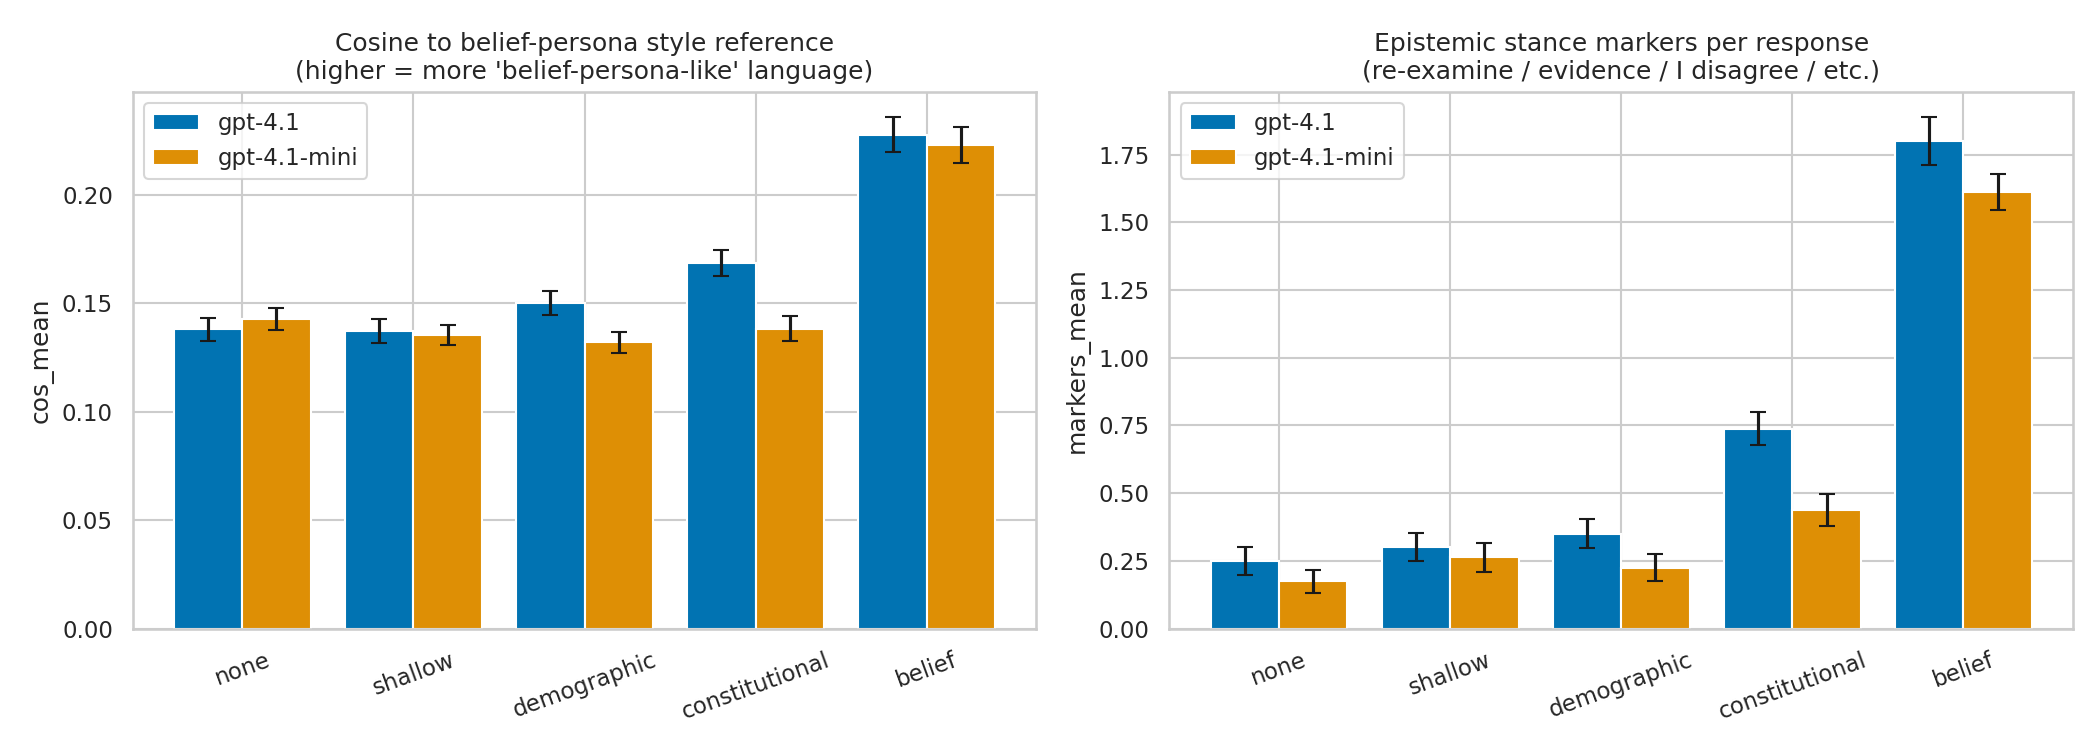
\includegraphics[width=0.95\linewidth]{figures/e3_persona_stickiness.png}
    \caption{Persona stickiness (\ethree). Left: cosine similarity between each response and a held-out belief-style reference paragraph (the reference was never used as a prompt). Right: count of epistemic-stance markers per response. The \pbelief condition is the only one whose responses cluster near the reference and the only one that produces \(>1\) stance marker per response on average.}
    \label{fig:e3}
\end{figure}

\begin{table}[t]
    \centering
    \begin{tabular}{@{}llrl@{}}
        \toprule
        \textbf{Model} & \textbf{Persona} & \textbf{Cosine to style ref.} & \textbf{Epistemic markers (mean \(\pm\) SD)} \\
        \midrule
        \gptone & \pnone & \(0.138\) & \(0.25 \pm 0.46\) \\
        \gptone & \pshallow & \(0.137\) & \(0.30 \pm 0.46\) \\
        \gptone & \pdemo & \(0.150\) & \(0.35 \pm 0.48\) \\
        \gptone & \pcai & \(0.169\) & \(0.74 \pm 0.55\) \\
        \gptone & \pbelief & \(\mathbf{0.228}\) & \(\mathbf{1.80 \pm 0.79}\) \\
        \midrule
        \gptmini & \pnone & \(0.143\) & \(0.18 \pm 0.38\) \\
        \gptmini & \pshallow & \(0.135\) & \(0.26 \pm 0.47\) \\
        \gptmini & \pdemo & \(0.132\) & \(0.23 \pm 0.45\) \\
        \gptmini & \pcai & \(0.138\) & \(0.44 \pm 0.52\) \\
        \gptmini & \pbelief & \(\mathbf{0.223}\) & \(\mathbf{1.61 \pm 0.61}\) \\
        \bottomrule
    \end{tabular}
    \caption{\ethree persona-stickiness measures. Best per model in \textbf{bold}. The \pbelief condition is the only one whose response embeddings cluster near the held-out belief-style reference (Welch \(t > 5.9\), \(p < 10^{-8}\), Cohen's \(d \geq 1.27\) vs \pnone, \(d \geq 0.94\) vs the strongest non-belief alternative).}
    \label{tab:e3}
\end{table}

The persona that produced the largest behavioral effect in \etwo is also the only persona whose surface style sticks. \Tabref{tab:e3} and \figref{fig:e3} show that the \pbelief condition has \(\sim 1.5\times\) the cosine similarity to the held-out reference as any other condition, and \(5\)--\(10\times\) more epistemic-stance markers per response than non-principled conditions. All \pbelief-vs-other contrasts on cosine are highly significant (Welch \(t > 5.9\), \(p < 10^{-8}\), Cohen's \(d \geq 1.27\) vs \pnone). The combination of \etwo and \ethree is the action-control claim: persona moves both surface (\ethree) \emph{and} behavior (\etwo), and they move together.
